\chapter{Design}

In this chapter, we introduce our tool Psnodig, and relevant design decisions. We also describe the design behind the Gourmet programming language, and the programs generating TBP and IBP.

\section{Proposed solution}

To solve the problem we are dealing with, we introduce Psnodig. We believe that Psnodig offers something unique in the context of this problem. Psnodig is a transpiler, intended to convert executable source programs to presentation-only target programs. \hfill \\

The programs discussed in Chapter 3 all do a very good job in their own right. The effort invested by developers, researchers and others involved is clearly reflected in both functionality and performance in each application. \hfill \\

However, none of them are particularly modifiable. We believe that a tool that combines these measures would be of even greater benefit. This way, the user does not have to operate with multiple tools at the same time. The user should also be able to add their own preferred output targets.

\forsup{``modifiable'' er ikke ordet jeg leter etter her. men kommer ikke på noe bedre akkurat nå..}

Additionally, these tools provide only the final result of conversion in the form of a PDF. We believe that the user would benefit from being able to modify the final result, in case the transition from the intermediate representation to the target is too lossy. \hfill \\

Where the programs primarily specialise in code generations, the DSLs are not executable. We believe that this is something that can be tremendously useful, and have therefore corporated an interpreter that works on the internal representation of Psnodig. To the best of our knowledge, a tool which combines all these methods does not currently exist. \hfill \\

Lastly, code generators traditionally do much more than directly translating data types to the target language. Therefore, we will refer to these programs simply as \textbf{writers} in the context of Psnodig, for the remainder of the thesis. \hfill \\

\forsup{Det er visstnok overraskende enkelt å skulle release Psnodig. Fikse noe cabal-greier og legge det ut på github, så skal man kunne kjøre `stack install`, og deretter skrive ting som `psnodig --tbp program.gt` istedenfor `stack run -- "--tbp" "program.gt"`!}

\section{Psnodig}

Psnodig is a collection of data types in Haskell, describing a computer program. As such, it does not provide a lot of functionality on its own. It is first when we add parsers and writers that it shows its usefulness. \hfill \\

Since we are free to add parsers and writers at will, only our imagination (and programming skills) can limit what we use it to convert. However, it is first and foremost intended as a tool for converting executable source programs to a presentation-only target programs. \hfill \\

To utilise Psnodig, source programs are parsed to an intermediate, internal representation. Later, this representation is used to convert the original program further into a new target program. This means that all source programs can be converted to the same target programs. \hfill \\

Psnodig also comes with an interpreter, which works on the internal representation. This means that we can add parsers and run the code, without having to write an additionaly interpreter or compiler. \hfill \\

The main benefit is that we can write our code once in a source language, test it, and when we are satisfied, transpile it to TBP and/or IBP thorugh the command line, rather than having to re-write it manually or search for a tool that can do that job for us. \hfill \\

\subsection{Syntax}

\forsup{blir egentlig syntax riktig ord å bruke her?}

The data types of Psnodig are presented in Listing ??. The entry point of a Psnodig program is \texttt{Program}, but since it consists of two lists and a \texttt{Maybe} data types, a minimal working example is actually an empty file. This flexibility allows our parsers and writers to utilise just as much, or as little, of the Psnodig syntax as we wish. \hfill \\

Most of the syntax will resemble the syntax of common programming languages. However, there are two statements that have been introduced specifically for Psnodig's real use case: Hash- and Annotation statements. \hfill \\

\begin{lstlisting}[caption={Psnodig's data types in Haskell}, captionpos=b, frame=trbl]
    data Program = Program [StructDecl] [Function]
                   (Maybe FunctionCall)

    data StructDecl = StructDecl String [Argument]

    data Struct = Struct String [Expression]

    data StructField = StructField Expression
                       Expression

    data Function = Function String [Argument]
                    [Statement]

    data FunctionCall = FunctionCall String
                        [Expression]

    data Argument = Argument String String

    data Statement =
          Assignment AssignmentTarget AssignmentValue
        | Loop Expression [Statement]
        | If Expression [Statement] (Maybe Else)
        | ForEach String Expression [Statement]
        | For String Expression Expression [Statement]
        | CallStmt FunctionCall
        | Return Expression
        | HashStmt Statement
        | AnnotationStmt String [Statement]
        | Break
        | Continue

    data AssignmentTarget =
          VariableTarget String
        | ListIndexTarget String [Expression]
        | StructFieldTarget StructField

    data AssignmentValue =
          ExpressionValue Expression
        | StructValue Struct

    data Else =
          ElseIf Expression [Statement] (Maybe Else)
        | Else [Statement]

    data Expression =
          Constant Value
        | VariableExp String
        | BinaryExp Operator Expression Expression
        | ListIndex String [Expression]
        | CallExp FunctionCall
        | Not Expression
        | StructExpr Struct
        | StructFieldExp StructField

    data Operator =
          Plus
        | Minus
        | Times
        | Division
        | LessThan
        | LessThanEqual
        | GreaterThan
        | GreaterThanEqual
        | Equal
        | NotEqual
        | And
        | Or
        | Modulo

    data Value =
          Nil
        | Boolean Bool
        | Number Integer
        | Text String
        | List [Expression]
        | HashSet (Set.Set Expression)
        | HashMap (Map.Map Expression Expression)
        | StructVal [(String, Value)]
\end{lstlisting}

Hash statements are statements intended to be parsed by the interpreter, but ignored by the writers. This lets us abstract away things that should be obvious to our audience, or perhaps things that have already been stated elsewhere, but still need to be stated for our programs to actually run. The name derives from how we can write single line comments in Python with a hash symbol. \hfill \\

A common use case of this is when a lower case \texttt{n} is often used to denote amounts in TBP. By using a hash statement, we avoid including superflous function calls to length-functions when it is obvious what \texttt{n} symbolises. \hfill \\

Annotation statements are statements that allow us to add an extra layer of abstraction to our output targets. The first string is what is presented, in natural language, whilst the list of statements is read by the interpreter. \hfill \\

A common use case of this is when we wish to swap two elements in a list. In many programming languages, when swapping two elements \texttt{a} and \texttt{b}, we have to assign \texttt{a} to a temporary variable, before assigning \texttt{a} to \texttt{b}, and finally assigning \texttt{b} to that temporary variable. These three implementation-specific lines could easily be abstracted with \texttt{swap a and b}. \hfill \\

These two statements are particularly useful when a piece of code is not crucial to the program's logic, or when the code is very implementation specific. The statement list can also be empty, which lets us explain things solely with natural language when deemed necessary. \hfill \\

\subsection{Interpreter}

A big selling point of Psnodig, is that in addition to being a transpiler, it also comes with an interpreter, which works on the AST. For a program to be transpiled, it only needs to be syntactically correct. However, this does not guarantee that the program works as the user intended. Thus, Psnodig provides users with the ability to test their programs before they are transpiled and later presented, which in many cases can be crucial. \hfill \\

Take the program presented in Listing ?? as an example. The function \\ \texttt{printEvenNumbers} takes two arguments: a list of numbers and the list's length. Then we iterate through this range, and proceed to print every number in the list that is even. However, we check for evenness by doing \texttt{if i \% 2 == 0}, but really we intend to do \texttt{if numbers[i] \% 2 == 0}. The difference is subtle, but by running the program we quickly realise the error when the screen displays 47, 79 and 93 rather than 46 and 22. \hfill \\

\begin{lstlisting}[caption={A syntactically correct program with a subtle logical error}, captionpos=b, frame=tlrb]{Name}
func printEvenNumbers(numbers list, length int) {
    for i := 0, length-1 {
        if i % 2 == 0 {
            print(numbers[i])
        }
    }

    return 1
}

printEvenNumbers([47, 46, 79, 22, 93], 5)
\end{lstlisting}

As seen from the grammar in Listing 4.1, programs consist of three parts: A list of struct declarations (which can be empty), a list of function declarations (which can also be empty), and lastly, an optional function call. The function call works as the entry point of the interpreter.

\subsubsection{Scope}

Psnodig works with both a global and a local scope. All structs and functions are global, and can be accessed from any other functions. For instance, functions can be mutually recursive. Variables, on the other hand, are always local, and a variable declared in function \texttt{f} cannot be accessed in function \texttt{g}, unless passed as an argument. \\

Listing ?? shows two syntactically valid programs, but Listing ?? (a) will yield an error, whilst Listing ?? (b) will eventually return 1. \\

\begin{minipage}{.45\textwidth}
\begin{lstlisting}[caption=Code with error, captionpos=b, frame=tlrb]{Name}
func f() {
    n := 5
    return g()
}

func g() {
    return n
}

f()
\end{lstlisting}
\end{minipage}\hfill
\begin{minipage}{.45\textwidth}
\begin{lstlisting}[caption=Code without error, captionpos=b, frame=tlrb]{Name}
func f() {
    n := 5
    return g(n)
}

func g(n int) {
    return n
}

f()
\end{lstlisting}
\end{minipage}

Psnodig supports nested scopes as indicated in the \texttt{For String Expression Expression [Statement]} structure within the \texttt{Statement} data type. The two \texttt{Expression} data types define a range, whilst the \texttt{String} data type serves as an identifier that binds to all numbers within this specified range (inclusive). \\

The statements are then executed repeatedly for each value in this range, with the identifier reflecting the current value on each iteration. Once the loop terminates, the identifier is automatically unbound, and no longer exists in the context.

\subsubsection{Peculiarities}

As seen, Psnodig prohibits two types of for loops. \texttt{For String Expression [Statement]} is discused in the previous subsection, but we also have \texttt{ForEach String Expression [Statement]}.

\forsup{Jeg vil egentlig endre dette til å være ForEach String Iterable [Statement], også begrenser vi Iterable til Variabler og ListIndex}

\subsubsection{Standard Library}

The interpreter provides several built-in functions, which are also found in most programming languages. They are also reflected in the TBP writer. If the function call fails, due to e.g. wrong number of arguments or arguments having the wrong type, the program will stop and the user will receive an explanatory error message. \\

\textbf{print($x_{1}$, $..$, $x_{n}$)}, which takes $n \in \mathbb{N}$ arguments. The arguments must be of type \texttt{Expression}, and each argument is printed on their own line in terminal. The function returns the number of arguments passed to it. \\

\textbf{length($x$)}, which takes one argument. The argument must be either a \texttt{Text}, \texttt{List}, \texttt{HashSet}, or \texttt{HashMap}. The function returns the length of its argument: Number of characters in text, number of elements in list and hashset, and number of mappings in hashmap. \\

\textbf{ceil($n$)} and \textbf{floor($n$)}, which take one number $n \in \mathbb{Q}$ as argument. The return value will be rounded up or down to the nearest $n' \in \mathbb{N}$, respectively. \\

\textbf{min($n_{1}$, $..$, $n_{n}$)} and \textbf{max($n_{1}$, $..$, $n_{n}$)}, which takes $m \in \mathbb{N}$ arguments. The arguments themselves must also be an $n \in \mathbb{N}$. The return value will be the smallest value and the largest value, respectively, amongst the arguments. \\

\textbf{append($x$, $xs$)}, which takes two arguments. The first argument must be an \texttt{Expression}, and the second argument must be a \texttt{List}. The function will append \texttt{x} to the end of \texttt{xs}, thus modifying the list. The function returns the number 1 if everything went well. \\

\textbf{add($x$, $hs$)} and \textbf{add($k$, $v$, $hm$)}, which is an overloaded function, taking either two or three arguments. In the first case, it adds an \texttt{Expression} $x$ to a \texttt{HashSet} $hs$. In the other case it maps an \texttt{Expression} $k$ to an \texttt{Expression} $v$ in a \texttt{HashSet} $hm$. The function always returns 1 upon success. \\

\textbf{get($k$, $hm$)}, which takes two arguments, an \texttt{Expression} $k$ and a \texttt{HashMap} $hm$. If $k$ is a key in $hm$, the function will return the value that $k$ maps to in $hm$. \\

\forsup{mangler: ``in'', for å sjekke for membership. kan brukes i sets, maps, lister og text}

\subsection{Testing}

Psnodig is not accompanied by any testing framework, but we have done some testing with QuickCheck \hfill \\

\forsup{Har ingen tester akkurat nå. Prøvde å teste 'AST -> Gourmet -> AST' tidligere, men la det på is. Kan det være en fin ting å teste?}

\forsup{en annen ting som kan være interessant å teste: programmer som transpiler til latex, uten å krasje. opplever noen ganger at jeg har glemt en edge case eller noe, eller til og med glemt å importere et bibliotek. vet ikke helt hvordan denne testen skulle sett ut, men det gir jo grunnlag for å si at det er ``trygt'' å bruke psnodig, og at det er ``komplett'' i konteksten av seg selv}

\section{Gourmet}

To make sure Psnodig works at all, we depend on having at least one input target and one output target. When it comes to input language, we have two plausible alternatives: Use an existing programming language, or design a new one. We decided to opt for the latter. \hfill \\

In the context of Psnodig, we just need to build a parser that can translate programs in the source language to the intermediate representation. There are several reasons as to why designing a new language for the purpose of proof of concept is a good choice. \hfill \\

For one, it demonstrates the general effort to add an entirely new input target for Psnodig. This can motivate others to add their own. Because the  \hfill \\

Another reason is that selecting a single programming language to encompass all needs is not feasible. For instance, the largest university in southern Norway uses Python for its introductory programming course\footnote{Course page for \textit{Introduction to object-oriented programming} at the University of Oslo:~\url{www.uio.no/studier/emner/matnat/ifi/IN1000/}}, whilst the largest university in northern Norway prefers C\footnote{Curriculum for \textit{Introduction to programming and the computer's mode of operation} at the University of Tromsø:~\url{www.bibsys-c.alma.exlibrisgroup.com/leganto/readinglist/lists/10569365600002205?institute=47BIBSYS_UBTO&auth=SAML}}. The largest university in Greece opts for Java~\footnote{Course page for \textit{Introduction to Computer Science} at the University of Athens:~\url{www.dept.aueb.gr/en/dmst/content/introduction-computer-science}}, and Harvard's renowned CS50 course introduces students to both JavaScript and SQL\footnote{Course page for \textit{Introduction to Computer Science} at the University of Harvard:~\url{www.pll.harvard.edu/course/cs50-introduction-computer-science}}. \hfill \\

\forsup{Lars kommenterte en gang at en fotnote burde ligge på utsiden høyresiden av punktum. Gjelder det også over her? er det bedre med feks ``tekst her og tekst der.1 2'' istedenfor ``tekst her 1 og tekst der 2.''? hvis det ga mening}

What the languages of introductory courses to computer science do have in common, is that they tend to be within the imperative paradigm of computer programming. As such, we did not want to stray too far away from that, and have allowed ourselves to mainly be inspired by the Go programming language. The language started out as a pure subset of Go, hence its name: A gourmet portion of Go.

\subsection{Lexical Aspects}

\subsubsection{Identifiers and keywords}

An identifier in Gourmet is used to reference either a struct, function or variable. Identifiers are also restricted to begin with a letter, followed by an arbitrary number of letters, numbers, and single quotes. \textbf{variable}, \textbf{var1able’} and \textbf{g0urmetVar1able''’'} are all valid Gourmet identifiers, whilst \textbf{1variable} and \textbf{'variable} are both not. Additionally, an identifier can not shadow keywords. \hfill \\

In total, there are 40 keywords in Gourmet, with 14 of them sharing structures with identifiers. They are \textbf{while}, \textbf{if}, \textbf{func}, \textbf{true}, \textbf{false}, \textbf{return}, \textbf{else}, \textbf{for}, \textbf{break}, \textbf{continue}, \textbf{struct}, \textbf{not}, \textbf{map} and \textbf{set}. These keywords are also reserved, which means that we cannot define an identifier \textbf{while} or \textbf{func}. The remaining keywords will be presented in Section ?? \hfill \\

We can define functions which clashes with library functions in Psnodig, but when trying to run that program, we receive an error message when our program tries to call those functions. This will happen even if we overload our functions with a different number of arguments, thus in reality removing the ambiguity. That means that we cannot run our own \textbf{print} function. However, we can always define a function e.g. \textbf{print’} or \textbf{print1}. \hfill \\

\subsubsection{Comments}

As there are no data types for comments in Psnodig, they must be handled entirely by Gourmet. The language supports both single- and multi-line comments, both identical to the ones found in most C-like languages like C itself, Java, Go and more. \hfill \\

Single-line comments begin with a double forward slash \textbf{//}, and extends to the end of that line. Multi-line comments start with a forward slash and a star \textbf{/*}, and end with a star and a forward slash \textbf{*/}. Multi-line comments cannot be nested, which means that the first \textbf{*/} after a \textbf{/*} will end that comment, no matter how many \textbf{\*} preceeds it. \hfill \\

\subsubsection{Whitespace}

Whitespace can be defined as spaces, newlines and tabs. Gourmet does not differentiate between either of them, and we can use them in our programs exactly how we wish. \hfill \\

Listing 4.1, Listing 4.2 and Listing 4.3 show a semantically identical program. We define a function \textbf{f} which again defines \textbf{a} to be a list with two elements, before returning it. Lastly, the fuction is called. All three programs will be successfully parsed, and have the same internal representation in Psnodig. \hfill \\

\begin{lstlisting}[caption={f with a standard amount of whitespace}, captionpos=b, frame=tlrb]
    func f() {
        a := [1, 2]
        return a
    }

    f()    
\end{lstlisting}

\begin{lstlisting}[caption={f with a lot of whitespace}, captionpos=b, frame=tlrb]
    func f()
    {
        a       :=
            [1   ,   2]
        return
        a
    }
    
    f   (   )
\end{lstlisting}

\begin{lstlisting}[caption={f with no whitespace}, captionpos=b, frame=tlrb]
    funcf(){a:=[1,2]returna}f()
\end{lstlisting}

\forsup{har tatt mye inspirasjon herfra: \url{https://github.uio.no/compilerconstruction-inf5110/compila/blob/master/doc/languagespec/compila.pdf} uten å kildeføre noe. her er jeg veldig usikker på hva jeg skal gjøre! har jeg kopiert for mye? KAN jeg i det hele tatt kildeføre noe slikt?}

\subsection{Types}

Gourmet is dynamically typed, which means that we do not have to specify the type of variables and return type of functions. In fact, Gourmet does not even \textit{allow} it. When defining structs and function arguments, however, we have to provide type hints on the form \textbf{name \textit{type}}. \hfill \\

The reason behind this choice is solely to improve code readability. When defining a variable, the value will always be present on the right hand side. When working with function arguments, however, we can never be entirely sure what a user decides to pass. With type hints, their ``intended use'' instantly becomes clear. \hfill \\

There are, however, four base types that all values will have: \textbf{Boolean}, \textbf{Number} and \textbf{Text}, and \textbf{nil}. A boolean is either true or false, a number is an arbitrarily large number, and a text is an arbitrarily combination of letters within a pair of double quotes. Nil indicates the absence of a value, and is mostly assigned as a placeholder. \hfill \\

Essentially, types associate data values into classes and provide rules for how these classes should interact[kilde]. Sometimes - to solve specific problems - the base types Gourmet offers might not suffice. Therefore, we can create our own types through structs. Structs in Gourmet work exactly the same way they do in languages like C and Go, containing instance variables, but no methods or constructors, like in languages like Python and Java. \hfill \\

Listing 4.4 shows how we can create a struct for modelling a tree data structure, and Listing 4.5 shows how they can be initialised. \hfill \\

\begin{lstlisting}[caption={A Gourmet struct Tree, with instance variables value, left and right}, captionpos=b, frame=tlrb]
    struct Tree {
        value int,
        left Tree,
        right Tree
    }
\end{lstlisting}

\begin{lstlisting}[caption=A function to initialise three tree structs and return the last one,captionpos=b, frame=tlrb]{Program}
    func f() {
        tree := struct Tree(10, nil, nil)
        tree' := struct Tree(20, nil, nil)
        tree'' := struct Tree(15, tree, tree')
        return tree''
    }
\end{lstlisting}

\subsection{Syntax}

\subsubsection{Grammar}

Gourmet's EBNF grammar is presented in Figure ??. EBNF (short for Extended Backus-Naur form) is a notation for expressing a programming language's grammar. It is an extension of BNF (short for Backus-Naur form) that was developed in the 1960s to describe the syntax of the ALGOL programming language [kilde]. We could have used the original BNF notation, but EBNF allows us to present it more succinctly. \hfill \\

In this variant of EBNF, we use the following meta symbols:

\begin{lstlisting}
    -> { } [ ] " ( ) |
\end{lstlisting}

Arrows indicate the application of a rule. Curly brackets indicate repetition of 0 or more times (much like the reflexive arrow in Figure 2.1). Square brackets indicate binary presentness. Vertical bars indicate option. Anything wrapped in double quotes is a keyword. \hfill \\

Non-terminals are written in upper case. There are also four terms written in upper case, that do not have production rules: \textbf{NAME}, \textbf{TEXT}, \textbf{NUMBER}, \textbf{STRING\_LITERAL}. NAME is an identifier, already described in Section 4.3.1.1. TEXT is any combination of UFT-8 symbols. It is only present once, and is intended for ``hiding'' code under an abstracting layer of natural language. NUMBER is any combination of whole numbers. STRING\_LITERAL is similar to TEXT, but additionally it is wrapped in double quotes. \hfill \\

\forsup{Bør jeg forklare dette mer? F.eks. dette med terminals og non-terminals osv.}

\begin{figure}
    \begin{subfigure}[ht]{1\linewidth}
        \begin{tabular}{c}
            \begin{lstlisting}
PROGRAM          -> { STRUCTDECL } { FUNCTIONDECL }
                    [ FUNCTIONCALL ]

STRUCTDECL       -> "struct" NAME "{" { ARGUMENT } "}"

FUNCTION         -> "func" NAME "(" [ ARGUMENT { ","
                    ARGUMENT } ] ")" "{" { STATEMENT }
                    "}"
ARGUMENT         -> NAME NAME

STATEMENT        -> ASSIGNMENT | LOOP | IF | FOREACH
                    | FOR | FUNCTIONCALL | ANNOTATIONSTMT
                    | # STATEMENT | "return" EXPRESSION
                    | "break" | "continue"

ASSIGNMENT       -> ASSIGNMENTTARGET ":=" ASSIGNMENTVALUE

LOOP             -> "while" EXPRESSION "{" { STATEMENT } "}"

IF               -> "if" EXPRESSION "{" { STATEMENT } "}"
                    [ ELSE ]

FOREACH          -> "for" NAME ":=" EXPRESSION "{"
                    { STATEMENT } "}"

FOR              -> "for" NAME ":=" EXPRESSION ","
                    EXPRESSION "{" { STATEMENT } "}"

FUNCTIONCALL     -> NAME "(" EXPLIST ")"

ANNOTATIONSTMT   -> "@" "{" TEXT "}" "{" { STATEMENT } "}"

ASSIGNMENTTARGET -> NAME | LISTINDEX | STRUCTFIELD

ASSIGNMENTVALUE  -> EXPRESSION | STRUCT

ELSE             -> "else" IF | "else" "{" { STATEMENT } "}"

EXPRESSION       -> VALUE | NAME | LISTINDEX
                    | EXPRESSION OPERATOR EXPRESSION
                    | FUNCTIONCALL | "not" EXPRESSION
                    | STRUCT | STRUCTFIELD

LISTINDEX        -> NAME "[" EXPRESSION "]" { "["
                    EXPRESSION "]" }

OPERATOR         -> "+" | "-" | "*" | "/" | "<" | "<="
                    | ">" | ">=" | "==" | "!=" | "&&"
                    | "||" | "%"

            \end{lstlisting}
        \end{tabular}
    \end{subfigure}
    \label{fig:gourmet-grammer1}
\end{figure}

\begin{figure}
    \begin{subfigure}[ht]{1\linewidth}
        \begin{tabular}{c}
            \begin{lstlisting}
STRUCT           -> NAME "(" EXPLIST ")"

STRUCTFIELD      -> EXPRESSION "." EXPRESSION

VALUE            -> "nil" | "true" | "false" | NUMBER
                    | STRING_LITERAL | "[" EXPLIST "]"
                    | "map" "{" [ PAIR { "," PAIR } ] "}"
                    | "set" "{" EXPLIST "}"

PAIR             -> EXPRESSION ":" EXPRESSION

EXPLIST          -> [ EXPRESSION { "," EXPRESSION } ]

            \end{lstlisting}
        \end{tabular}
    \end{subfigure}
    \setcounter{figure}{1}
    \caption{The EBNF grammar of the Gourmet programming language}
    \label{fig:gourmet-grammer1}
\end{figure}

\subsubsection{Precedence and Associativity}

The precedence of Gourmet operators is ranked in the following order, from highest to lowest:

\begin{enumerate}
    \item $*$ and $/$ and $\%$
    \item $+$ and $-$
    \item $<$, $<=$, $>$ and $>=$
    \item $==$ and $!=$
    \item $\&\&$ and $||$
    \item $.$ (to access fields of a struct)
    \item not
\end{enumerate}

This means that if we wish to calculate the sum of the tree values from Listing 4.5, we cannot write \texttt{tree.value + tree'.value + tree''.value}, because the parser will parse \texttt{(p.(value + p').(value + p'')).value}. Therefore, we have to include parentheses explicitly: \texttt{(tree.value) + (tree'.value) + (tree''.value)}. \hfill \\

All binary operations are left-associative.

\section{TBP Writer}

Our TBP writer takes an internal representation of Psnodig and produces a LaTeX file. As previously stated, we are not attempting to create a ground truth for pseudocode. Therefore, we have chosen to produce the pseudocode with the Algorithm2e package. \hfill \\

\forsup{Akkurat nå håndterer vi ikke Input, Output og Caption. Hvordan dette gjøres er nok ikke så farlig. Må bestemme om dette skal bakes inn i Psnodig, eller om vi f.eks. skal hente det fra kommandolinjen idet noen kjører ``stack run -- tbp program.gt''}

Structs and the initial function call are not converted to pseudocode. For one, we believe that function calls are rarely cruical to the algorithm itself, and structs will always be implementation specific. \hfill \\

\forsup{jeg sverger jeg hadde en til grunn}

\subsection{Algorithm2e}

\forsup{Bør jeg skrive en eller annen intro om pakken?}

Algorithm2e allows us to define our own keywords with the \texttt{\textbackslash SetKw\{\}\{\}} command. These are macros, where if we define \texttt{\textbackslash SetKw\{KwBreak\}\{break\}}, we can write \texttt{\textbackslash KwBreak}, and \texttt{break} will be printed. \hfill \\

There are also more specific macros, like \texttt{\textbackslash SetKwProg\{proc\}\{Procedure\}\{is\}\{end\}}. This is used to initialise programs, and denotes a special syntax for the program. Listing ?? (a) shows an example program, and Listing ?? (b) shows the subsequent compiled result. For our TBP writer, we decide to ignore the last two parameters, because we do not believe they add enough value to the final result. \hfill \\

\forsup{fiks eksempel til den over.}

Another special macro is \texttt{\textbackslash SetKwFunction\{f\}\{f\}}. This allows us to write e.g. \texttt{\textbackslash f\{arg1, arg2, arg3\}}, which looks like displays \f{arg1, arg2, arg3}. \hfill \\

Since we are still in a LaTeX environment, and backslashes are used for macros in standard LaTeX too, we have to be careful. We are not allowed to rename internal macros. For instance, \texttt{\textbackslash m} is already a macro in LaTeX, thus attempting to compile a file with \texttt{\textbackslash SetKwFunction\{m\}\{m\}} will lead to multiple errors and ruin the final output.

\subsection{Compatibility with Psnodig}

As previously mentioned in Section ??, all Psnodig library functions taken into consideration by our TBP writer. The function call \texttt{length(list)} is transpiled with the cardinality symbols to $\abs{list}$. The function call \texttt{append(x, xs)} is transpiled with natural language, to \texttt{append x to xs}, to avoid ambiguity. \\

Mathematical expressions are also taken into consideration. For instance, the Expression \texttt{BinaryExp Division (Constant (Number 2)) (Constant (Number 1))} will show $\frac{2}{1}$, rather than \texttt{2/1}. Similarly, an expression with multiplication will be displayed as \texttt{n $\cdot$ n} rather than \texttt{n * n}. \\

To work with mathematical symbols in LaTeX we use the packages \textbf{amsmath} and \textbf{commath}. \\

We also declare some macros to match the syntax of Psnodig. For instance, all programs come with \texttt{\textbackslash SetKw\{Return\}\{Return\}} and \texttt{\textbackslash SetKw\{False\}\{false\}}. Code like \texttt{return 5} or \texttt{v := false} will be presented with the keywords in boldface. \\

\forsup{Before a program is transpiled to TBP, another program is ran to see which keywords are used, and only these are imported in the resulting LaTeX file. So, unless the program actually contains a \texttt{Return} expression, the macro will not be included. This makes the program less bloated, and easier to navigate if the user wishes to modify something themselves.}

\subsection{Output}

Transpiling a program to TBP yields two files: a corresponding LaTeX file, and a PDF version of said LaTeX file. \\

Because the LaTeX file is built from Psnodig's internal representation, and not directly from the source program, formatting is not taken into account. This means that a program like

\texttt{ func f()\{v:=5 returnv\}f() } \\

will not be transpiled to \\

\texttt{ \textbackslash proc\{\$\textbackslash f()\$\}\{\$\textbackslash texttt\{v\}\textbackslash gets5\$\textbackslash ; \textbackslash Return\$v\$\textbackslash;\} } \\

but instead

\begin{verbatim}
    \proc{$\f()$}{
        $\texttt{v} \gets 5$ \;
        \Return $v$ \;
    }
\end{verbatim}

even though they would produce the same PDF. The LaTeX files also include \texttt{ \textbackslash SetKwProg\{proc\}\{Procedure\}\{\}\{\} } and \texttt{ \textbackslash SetKwFunction\{f\}\{f\} }. We include the \texttt{linesnumbered}- and \texttt{ruled} parameters from algorithm2e, purely for aesthetic reasons. Listing ?? (a) shows the program we just mentioned with these parameters, whilst Listing ?? (b) shows the same program without the parameters. \\

\begin{figure}[ht]
\centering
\begin{subfigure}{.5\textwidth}
  \centering
  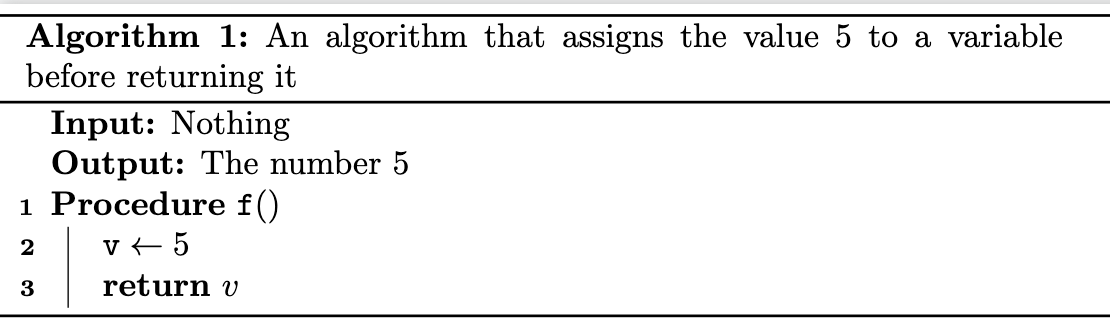
\includegraphics[width=.9\linewidth]{assets/return5pretty.png}
  \caption{f with extra parameters}
  \label{fig:sub1}
\end{subfigure}%
\begin{subfigure}{.5\textwidth}
  \centering
  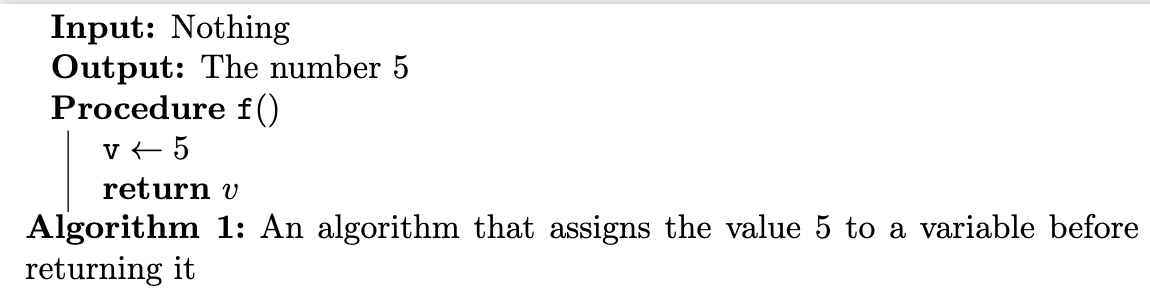
\includegraphics[width=.9\linewidth]{assets/return5ugly.png}
  \caption{f without extra parameters}
  \label{fig:sub2}
\end{subfigure}
\caption{TBP of an algorithm f, with and without extra visual parameters}
\label{fig:test}
\end{figure}

\forsup{If, for some reason, we do not want a PDF to accompany our LaTeX file, we can put an extra flag when calling the program. The flag is ``--nopdf'', and the whole command would be ``psnodig --tbp --nopdf program.gt''.}

\forsup{Burde jeg skrive noe om flagg og sånt i Design av Psnodig?}


\section{IBP Writer}

Our IBP writer works much like the TBP writer: An internal representation of Psnodig is transpiled to a LaTeX file. The flowcharts are created with the TikZ package. \\

Just like the TBP writer, our IBP writer only transpiles the topmost function, ignoring structs and the initial function call. Our reasoning is the same as earlier. To transpile a program to IBP, we run \texttt{psnodig --ibp <program>} in the command line.

\subsection{TikZ}

TikZ is a massive package. We actually used TikZ to create the FSA example in Section 2.1.2. \\

\forsup{Bør jeg skrive en eller annen intro om pakken?}

Our flowcharts mainly consist of three macros: \texttt{\textbackslash tikzstyle}, \texttt{\textbackslash node}, and \texttt{\textbackslash edge}. \texttt{tikzstyle} lets us choose what our nodes look like, \texttt{ndode} lets us draw the nodes we want, and \texttt{edge} lets us add an edge between nodes. \\

Each node in our flowcharts represents a statement, except the top one, which is the function name. The visual design is simple: the top node and all nodes of return statements are dark rectangles with rounded edges. Decision nodes, where the program diverges, are yellow diamonds. These are while-, for- and if-statements. The remaining statements are purple rectangles. The edges are thin arrows. \\

Tikzstyles are written on the form

\begin{verbatim}
    \tikzstyle {style name} =
        [ shape
        , minimum width = x cm
        , minimum height = y cm
        , text <position>
        , draw = colour
        , text = colour'
        , fill = colour''
        ]
\end{verbatim}

The style name will be referenced later by nodes. The shape can be a rectangle, circle or coordinate, but we can import more libraries to get shapes like e.g. diamonds. The three colours refer to the node's border-, text- and background colours, respectively. We have also opted to center all text. \\

Nodes are written on the form

\begin{verbatim}
    \node (unique name)
          [metadata]
          {text displayed on node}
\end{verbatim}

All nodes should have a unique name, so that they can be referenced correctly later. The square brackets denote metadata. For instance, how the node should look like (by referencing a tikzstyle), or the nodes positioning relative to other nodes. The curly brackets is the text displayed within the node area. \\

Edges are written on the form

\begin{verbatim}
    \draw [edge] (node) -- (node')
\end{verbatim}

The biggest issue with the TikZ package, is that we first have to write all of our nodes before adding edges between them. \forsup{This means that we must save all statements in a graph before printing them.}

When working with large control flow statements, we have to deal with multiple else-branches. Rather than following each other vertically, they are placed horizontally. \forsup{We calculate a reasonable distance, and place the nodes evenly}. An issue is that, nodes with a lot of text might interfere with each other. \\

\forsup{Eksempler?}

Additionally, having multiple straight edges from the same source might interfere with each of the edge labels. Thus, we might also have to change the way we draw edges, for instance like this

\begin{lstlisting}
    \draw [edge] (node) |- (node');
\end{lstlisting}

This will curve the edge between \texttt{node} and \texttt{node'}, making the flowchart clearer. This is, however, a difficult task to carry out since we never know how programs turn out. Therefore it seems natural to opt for the easiest choice available and instead, unfortunately, force the authors of tweaking the resulting LaTeX on their own. \\

\subsection{Compatibility with Psnodig}

\forsup{Jeg lar denne stå litt WIP, siden jeg ikke har kommet så langt}

\subsection{Output}

Just like TBP, transpiling a program to IBP yields both a LaTeX file and a PDF. Listing ?? shows the resulting LaTeX if we run \texttt{psnodig --ibp program} on the program from Section 4.4.3. It also shows how we position nodes vertically. \hfill \\

\begin{lstlisting}[caption={The LaTeX from transpiling a program to IBP}, captionpos=b, frame=trbl]
    \node (0) [startstop] {f()};
    \node (1) [statement, below of=0] {v = 5};
    \node (2) [startstop, below of=1] {v};

    \draw [edge] (1) -- (2);
    \draw [edge] (0) -- (1);
\end{lstlisting}